\documentclass[12pt]{article}

\usepackage{tabularx}
\usepackage[a4paper,margin=2.5cm, bottom=4cm]{geometry}
\usepackage{fancyhdr}
\usepackage{listings}
\usepackage{booktabs}
\usepackage{float}
\usepackage{subcaption}
\usepackage{graphicx}
\usepackage{amsmath}
\usepackage{amssymb}
\usepackage{amsthm}
\usepackage{array}
\usepackage[table]{xcolor}
\usepackage{pgfplots}
\usepackage{pgfplotstable}
\usepackage{multirow}
\usepackage{tikz}
\pgfplotsset{compat=1.17}

\theoremstyle{definition}
\newtheorem*{example}{Example}

\graphicspath{{../img_task1/}}

\setlength{\headheight}{40pt}
\setlength{\parindent}{0pt}
\setlength{\parskip}{1ex}
\renewcommand{\headrulewidth}{0pt}

\newcommand{\subfiguresize}{.3\textwidth}
\DeclareMathOperator*{\median}{median}

\lstset {
    basicstyle = \small\ttfamily,
    keywordstyle = \color{blue},
    commentstyle = \color{black!30},
    comment = [l]{//},
    morecomment = [s]{/*}{*/},
    identifierstyle=,
    keywords = {
        let,
        mut,
        for,
        in,
        if,
        else,
        pub,
        struct,
        impl,
        type,
        Self,
        u8,u16,u32,u64,
        i8,i16,i32,i64,
        f32,f64,
    }
}

\begin{document}

\pagestyle{fancy}
\fancyhead{}
\fancyhead[L]{
    \renewcommand{\arraystretch}{1.5}
    \begin{tabularx}{\textwidth}{|X|X|}
        \hline
        \large \bf Image processing & \normalsize Task No. 1 \\
        \hline
    \end{tabularx}
}
\fancyfoot[C]{\thepage}

\thispagestyle{empty}
\renewcommand{\arraystretch}{2}
\begin{flushleft}
    \begin{tabularx}{0.95\textwidth}{|X|X|}
        \hline
        \bf \large Image Processing                   & \bf \large Task No.~1                           \\ \hline
        \multicolumn{2}{|l|}{
            \textbf{Task variant:} Group 1
        }                                                                                               \\ \hline
        \textbf{Day and time:} Mon, 14:00             & \textbf{Full name:} \textsc{Jakub Pawlak}       \\
        \textbf{Academic year: 3\textsuperscript{rd}} & \textbf{Full name:} \textsc{Magdalena Paku\l a} \\
        \hline
    \end{tabularx}
\end{flushleft}
\vspace{1em}
\renewcommand{\arraystretch}{1}

\section{Technical description of the program}
\subsection{Basic information}

Technical description of the application
This application allows a user to apply some operations to images, which are:
\begin{enumerate}
    \item basic color correction operations such as modifying brightness or contrast
    \item geometric operations, for example resizing or flipping the image
    \item noise removal filters (in this case median and geometric mean)
\end{enumerate}
We decided to write our project in the Rust programming language due to its multiple advantages, such as:
high speed due to it being compiled language like C++, yet with much more safety mechanisms for managing memory without the use of a garbage collector.

To view the instructions of usage, the user should invoke the program with ``\lstinline{--help}'' argument.
This will print all of the available operations, including the arguments that the user should provide.
The basic format for all the operations are:
\begin{center}
    \lstinline{executable --command [-argument=value]* input_file}
\end{center}

\subsection{Advanced information}
\subsubsection{Used libraries}
The external libraries (called ``crates'' in case of Rust) that we use in our project are
\begin{itemize}
    \item \textbf{image} --- providing implementations of image encoders and decoders,
          used for reading and saving the images
    \item \textbf{vulkano} --- Rust wrapper around the Vulkan graphical API,
          which we use to provide alternative implementations of some transformations,
          which are run on the GPU making them significantly faster
    \item \textbf{vulkano-shaders} --- providing some macros that automatically,
          during the program's compilation,
          also compile the glsl shader code and embed it in the final binary.
\end{itemize}

\subsubsection{Data structures}
For storing the image we use RgbImage struct from the mentioned image crate,
which is just a wrapper around a vector of pixels, which in turn are just a 3-element array of unsigned 8-bit integers (one for each RGB channel).

\section{Description of implementation of basic image operations}

\paragraph*{Preface on the used notation}
In the equations we write to describe operations, we will use luminosity functions $f$ to describe the original image, and $\hat{f}$ to describe the new image (after transformation).
$f(x,y)$ will denote the luminosity of the pixel at the coordinates $x,y$. Unless explicitly stated, the method will be the same for each color channel.
For brevity, if the pixel coordinates are irrelevant, they may be ommited and be assumed to be the same for $\hat{f}$ and $f$, i.e.\ $\hat{f}=f$ is equivalent to $\hat{f}(x,y) = f(x,y)$.
Additionally, we define $x|_{[a,b]}$ as $x$ restricted to the range $[a,b]$, that is $\max\{a, \min\{x,b\}\}$.
For parameters that are specified by the user (e.g\ in brightness or contrast modifications), we will use letters from the greek alphabet.

\vspace{5em}
% \pagebreak[3]
\subsection{Brightness modification (B1)}

\subsubsection{Implementation}

For modyfying brightness we simply add the amount supplied by the user to the luminosity value of each pixel.
Because such operation can exceed the range of allowed values, we have to restrict the result to the range $[0,255]$.

\begin{equation}
    \hat{f} = (f + \alpha) \, \Big|_{[0,255]}
\end{equation}

\subsubsection{Results}

\begin{figure}[H]\centering
    \begin{subfigure}[t]{\subfiguresize}\centering
        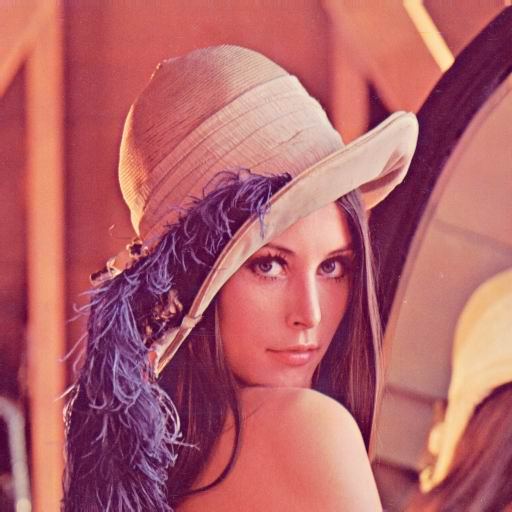
\includegraphics[width=\textwidth]{lenac.png}
        \caption{original}
    \end{subfigure}
    \hspace{.05\textwidth}
    \begin{subfigure}[t]{\subfiguresize}\centering
        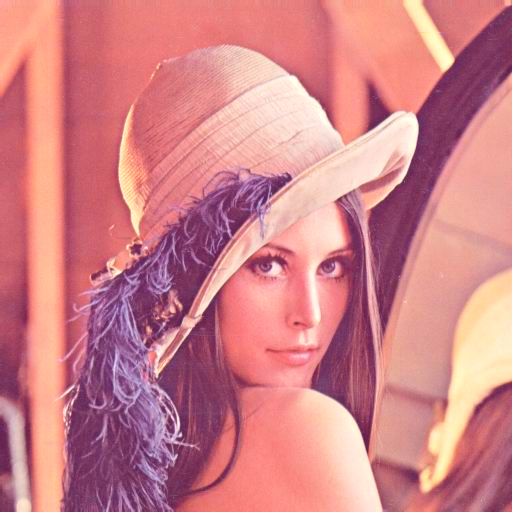
\includegraphics[width=\textwidth]{lenac_bright+30.png}
        \caption{with increased brightness}
    \end{subfigure}
    \caption{Image before and after increasing the brightness by 30}
\end{figure}

\subsubsection{Complexity analysis}

The operation for one pixel is of constant time,
therefore the total computational complexity for the image of size $w \times h$ is $\mathcal{O}(wh)$.
The algorithm operates in-place, therefore it's space complexity is $\mathcal{O}(1)$.

\vspace{5em}
\pagebreak[3]
\subsection{Contrast modification (B2)}

\subsubsection{Implementation}

For contrast modification, we want to multiply the luminosity values by the specified factor
in order to modify the slope of the tone curve.

However, plain multiplication would result in visible brighness modification alogside the contrast change.
We, however, would like to make the dark pixels darker, and bright ones brighter.
For this reason, we offset the input luminosity by 128, to produce rotation around the center.

\begin{figure}[ht]\centering
    \begin{tikzpicture}
        \begin{axis}[
                % width=.5\textwidth,
                height = .4\textwidth,
                xmin=0,
                xmax=255,
                ymin=0,
                ymax=255,
                xtick = {0,255},
                xlabel = {\small input},
                ytick = {0,255},
                ylabel = {\small output}
            ]
            \addplot[black,domain=0:255,dotted]{x};
            \addplot[blue,domain=0:255,thick]{min(x*2,254)};
            \addplot[red,domain=0:255,thick]{max(1,min((x-128)*2+128,254))};
            % should be clamped to [0,255], but we use [1,254] for better visibility
        \end{axis}
    \end{tikzpicture}
    \caption{Contrast modification ($\alpha = 2$) without offset (blue), and with offset (red)}
    \label{fig:contrast-differences}
\end{figure}

The difference is shown of fig. \ref{fig:contrast-differences}.
We can clearly see the benefit of using the offset, so for computation we will use the following formula:

\begin{equation}
    \hat{f} = \left((f - 128) \cdot \alpha + 128\right)\Big|_{[0,255]}
\end{equation}

\subsubsection{Results}

\begin{figure}[H]\centering
    \begin{subfigure}[t]{\subfiguresize}\centering
        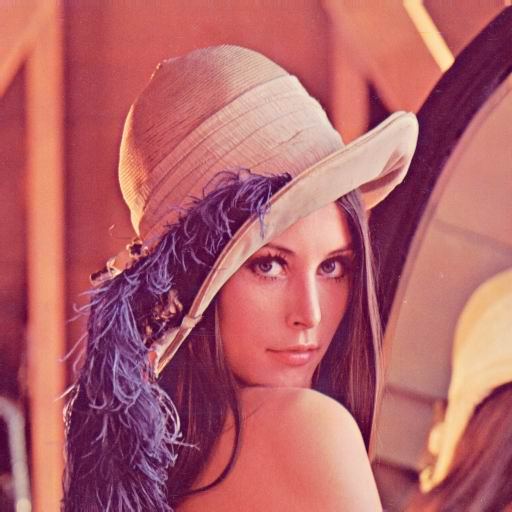
\includegraphics[width=\textwidth]{lenac.png}
        \caption{original}
    \end{subfigure}
    \hspace{.05\textwidth}
    \begin{subfigure}[t]{\subfiguresize}\centering
        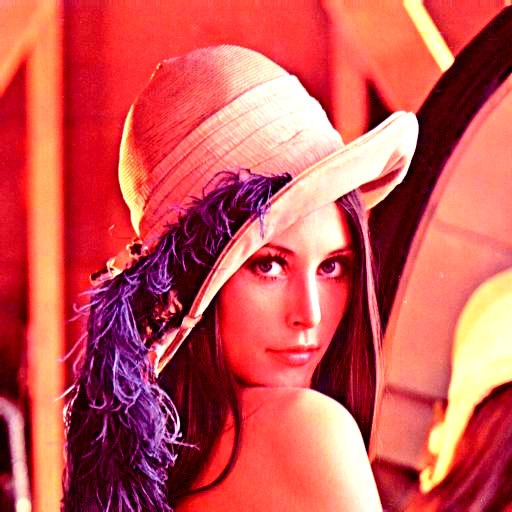
\includegraphics[width=\textwidth]{lenac_contrast_2x.png}
        \caption{with increased contrast}
    \end{subfigure}
    \caption{Image before and after increasing the contrast by a factor of 2}
\end{figure}

\subsubsection{Complexity analysis}

The operation for one pixel is of constant time,
therefore the total computational complexity for the image of size $w \times h$ is $\mathcal{O}(wh)$.
The algorithm operates in-place, therefore it's space complexity is $\mathcal{O}(1)$.

\vspace{5em}
\pagebreak[3]
\subsection{Negative (B3)}

\subsubsection{Implementation}

Negative is produced by subtracting each pixel from the maximum intensity value, resulting in a complementary color.
It can be expressed as the following equation:

\begin{equation}
    \hat{f} = 255 - f
\end{equation}

\subsubsection{Results}

\begin{figure}[H]\centering
    \begin{subfigure}[t]{\subfiguresize}\centering
        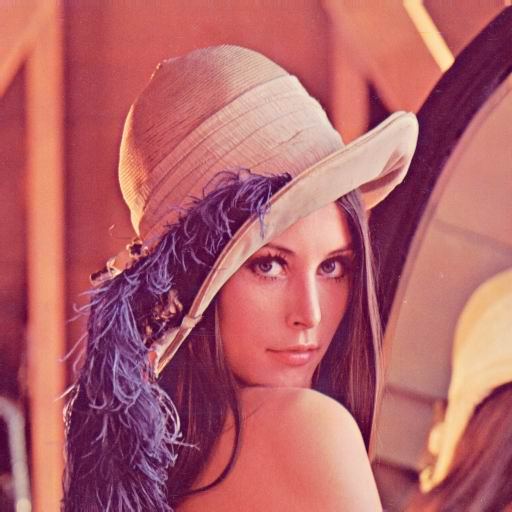
\includegraphics[width=\textwidth]{lenac.png}
        \caption{original}
    \end{subfigure}
    \hspace{.05\textwidth}
    \begin{subfigure}[t]{\subfiguresize}\centering
        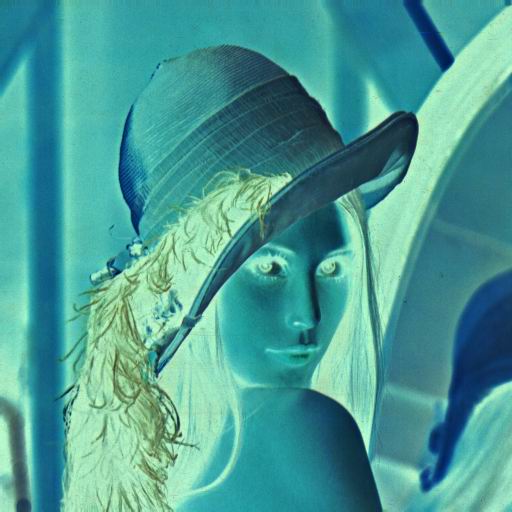
\includegraphics[width=\textwidth]{lenac_negative.png}
        \caption{negative}
    \end{subfigure}
    \caption{Image before and after inverting the colors}
\end{figure}

\subsubsection{Complexity analysis}

Similarly to the previous transformation,
the operation on one pixel is constant time, which for $w \times h$ pixels in total gives computational complexity $\mathcal{O}(wh)$
and space complexity $\mathcal{O}(1)$.

\vspace{5em}
\pagebreak[3]
\subsection{Horizontal flip (G1)}

\subsubsection{Implementation}

Horizontal flip performs a mirroring operation around the vertical axis.
Therefore, the $y$ coordinates will remain unchanged, and $x$ coordinates will be mirrored around the center.
\begin{equation}
    \hat{f}(x,y) = f(width - x, y)
\end{equation}

We accomplish this by looping over every pixel in the left half of the image,
and swapping it with it's mirror pixel.

We loop only over the left half
because otherwise, each pair of pixels would be swapped twice,
cancelling each other.

\subsubsection{Results}

\begin{figure}[H]\centering
    \begin{subfigure}[t]{\subfiguresize}\centering
        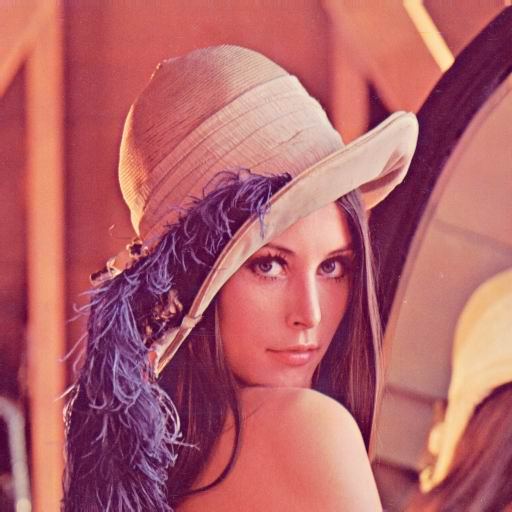
\includegraphics[width=\textwidth]{lenac.png}
        \caption{original}
    \end{subfigure}
    \hspace{.05\textwidth}
    \begin{subfigure}[t]{\subfiguresize}\centering
        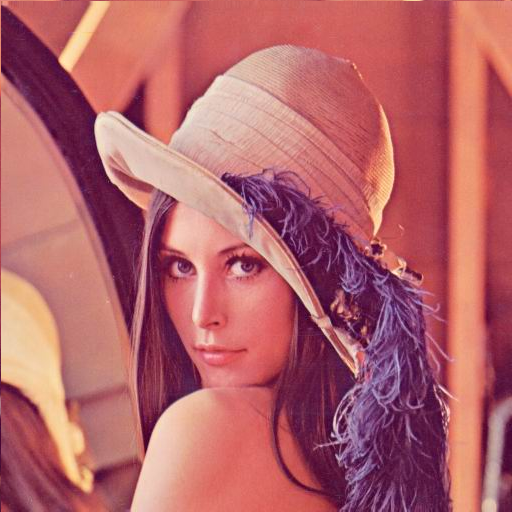
\includegraphics[width=\textwidth]{lenac_hflip.png}
        \caption{flipped}
    \end{subfigure}
    \caption{Image before and after flipping it horizontally}
\end{figure}

\subsubsection{Complexity analysis}

The operation for one pair of pixex is of constant time,
therefore the total computational complexity for the image of size $w \times h$ is $\mathcal{O}(\frac{wh}{2}) = \mathcal{O}(wh)$.
The algorithm operates in-place, therefore it's space complexity is $\mathcal{O}(1)$.

\vspace{5em}
\pagebreak[3]
\subsection{Vertical flip (G2)}

\subsubsection{Implementation}

The vertical flip works almost identically as the horizontal one,
except the mirror axis is horizontal, not vertical.
Therefore, the implementation is also almost identical.
The only difference is that instead of looping over the left half,
we loop over the top one, and the $x$ coordinate stays constant,
while the swap occurs at the $y$ coordinate

\begin{equation}
    \hat{f}(x,y) = f(x, height - y)
\end{equation}

\subsubsection{Results}

\begin{figure}[H]\centering
    \begin{subfigure}[t]{\subfiguresize}\centering
        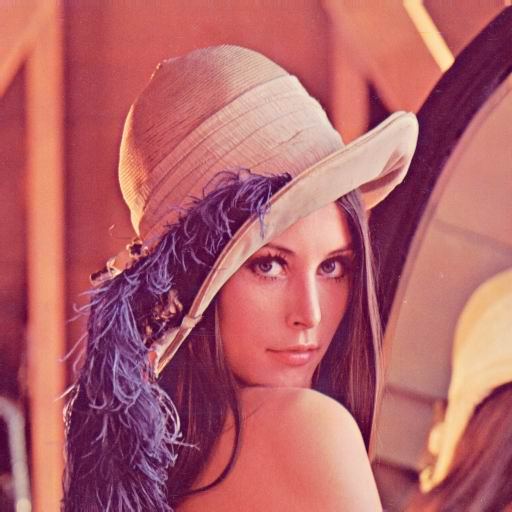
\includegraphics[width=\textwidth]{lenac.png}
        \caption{original}
    \end{subfigure}
    \hspace{.05\textwidth}
    \begin{subfigure}[t]{\subfiguresize}\centering
        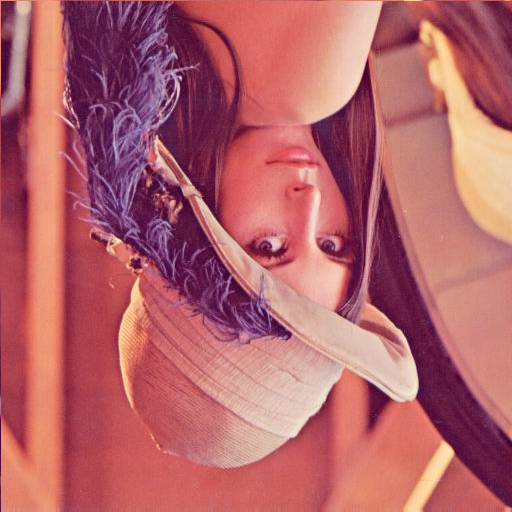
\includegraphics[width=\textwidth]{lenac_vflip.png}
        \caption{flipped}
    \end{subfigure}
    \caption{Image before and after flipping it vertically}
\end{figure}

\subsubsection{Complexity analysis}
Similarly to the horizontal flip,
the computational complexity is $\mathcal{O}(wh)$, and the spacial complexity is $\mathcal{O}(1)$.

\vspace{5em}
\pagebreak[3]
\subsection{Diagonal flip (G3)}

\subsubsection{Implementation}

The diagonal flip is just the vertical flip composed with the vertical flip.
The order of the composition does not matter.

\begin{equation}
    \hat{f}(x,y) = f(width - x, height - y)
\end{equation}

The implementation reflects the composition aspect,
instead of providing a custom implementation,
we just apply the 2 existing flips.

We are aware, that this is not the most optimal solution,
as we are unnecessarily looping over the pixels in both flips instead of just one,
however, this operation is still so quick,
that the performance degradation coming from using a suboptimal implementation
is not noticeable to the end user.

\subsubsection{Results}

\begin{figure}[H]\centering
    \begin{subfigure}[t]{\subfiguresize}\centering
        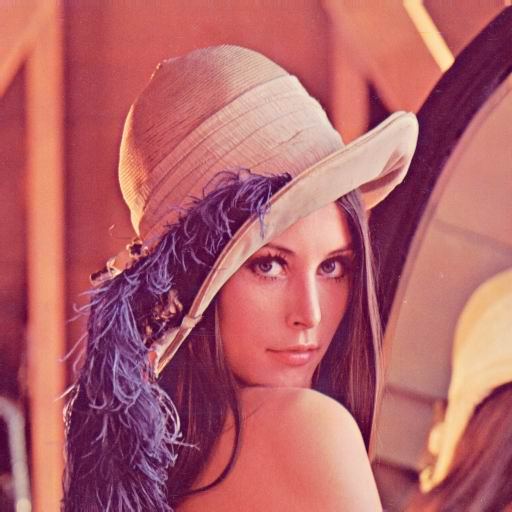
\includegraphics[width=\textwidth]{lenac.png}
        \caption{original}
    \end{subfigure}
    \hspace{.05\textwidth}
    \begin{subfigure}[t]{\subfiguresize}\centering
        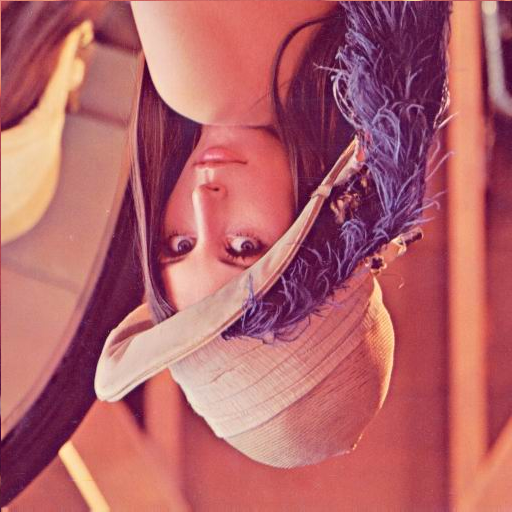
\includegraphics[width=\textwidth]{lenac_dflip.png}
        \caption{flipped}
    \end{subfigure}
    \caption{Image before and after flipping it diagonally}
\end{figure}

\subsubsection{Complexity analysis}
Since it is just applying two flips, each of which are $\mathcal{O}(wh)$,
the computational complexity is also $\mathcal{O}(wh)$, and the spacial complexity is $\mathcal{O}(1)$.

\vspace{5em}
\pagebreak[3]
\subsection{Shrink (G4) and Enlarge (G5)}

\subsubsection{Implementation}

For shrinking and enlarging, we will implement just one transformation, called scale.
Given some factors $\varphi_x, \varphi_y$ and an image with dimensions $w \times h$,
it will produce a new image of dimensions $\varphi_x w \times \varphi_y h$.
For handling cases where the pixels should be interpolated,
we chose to use floor function,
as it was not stated that we should use any specific method for handling such cases.
The choice of this method will result in a visible pixelation when scaling up by a large factor,
which may or not be desirable depending on the type of image
(for example this method will work very well with enlarging pixel-art style images, but less so with photographs).

\begin{equation}
    \hat{f}(x,y) =
    f\left(
    \left\lfloor
    \frac{x}{\varphi_x}
    \right\rfloor,
    \left\lfloor
    \frac{y}{\varphi_y}
    \right\rfloor
    \right)
\end{equation}

Although our function allows for different scaling factors
in the $x$ and $y$ dimensions,
the user is only able to input one value $\varphi$,
to preserve the original image aspect ratio,
so the program just sets $\varphi_x = \varphi_y = \varphi$.

Enlarge will just apply scale with the factor as it is, and shrink will apply scale, but with the inverse of the specified factor,
i.e.\ if we want to shrink by a factor of 2, we will apply scale with a factor of $\frac{1}{2}$.

\subsubsection{Results}

\begin{figure}[H]\centering
    \begin{subfigure}[t]{\subfiguresize}\centering
        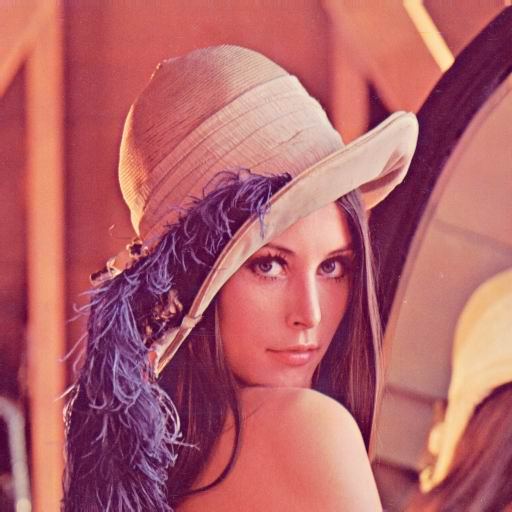
\includegraphics[width=\textwidth]{lenac.png}
        \caption{original ($512 \times 512$)}
    \end{subfigure}
    \hspace{.05\textwidth}
    \begin{subfigure}[t]{\subfiguresize}\centering
        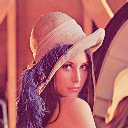
\includegraphics[width=.7\textwidth]{lenac_small.png}
        \caption{shrunk ($128 \times 128$)}
    \end{subfigure}
    \caption{Image before and after shrinking by a factor of 4 (not to scale)}
\end{figure}

\begin{figure}[H]\centering
    \begin{subfigure}[t]{\subfiguresize}\centering
        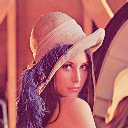
\includegraphics[width=.7\textwidth]{lenac_small.png}
        \caption{original ($128 \times 128$)}
    \end{subfigure}
    \hspace{.05\textwidth}
    \begin{subfigure}[t]{\subfiguresize}\centering
        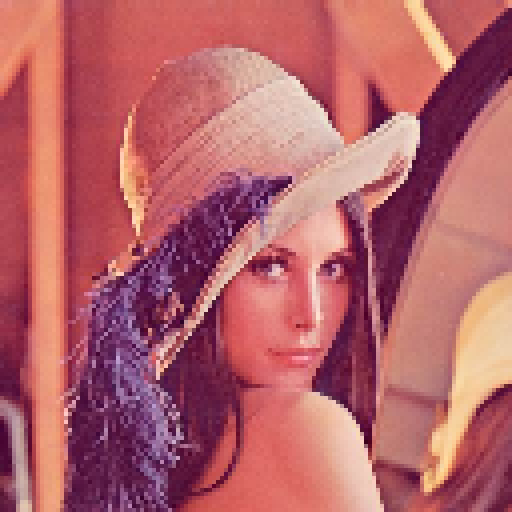
\includegraphics[width=\textwidth]{lenac_enlarged.png}
        \caption{enlarged ($512 \times 512$)}
    \end{subfigure}
    \caption{Image before and after enlarging by a factor of 4 (not to scale)}
\end{figure}

\subsubsection{Complexity analysis}

We loop over every pixel in the \emph{new image}, which has dimensions $\varphi w \times \varphi h$.
Therefore, the computational complexity is $\mathcal{O}(wh \varphi^2)$.

The spacial complexity is the size of buffer we need to allocate for the new image. Therefore it is $\mathcal{O}(wh \varphi^2)$.

\pagebreak
\section{Description of the implementation of the noise reduction methods}

\subsection*{Common implementation}
We noticed that all the filters operate by gathering some neighbourhood around the target pixel,
and then applying some reducing function on that pixels to determine the value of the resulting pixel.
Therefore, in order to remove duplication, we extracted the common functionality
of gathering the pixels to a special struct called \lstinline{Neighbourhood}, which holds a reference to the image, and the bounds of the neighbourhood.

\begin{lstlisting}
pub struct Neighbourhood<'a> {
    image: &'a RgbImage,
    min_x: u32,
    max_x: u32,
    min_y: u32,
    max_y: u32,
}
\end{lstlisting}

Let $Img$ denote some image, and $w$ and $h$ the width and height of $Img$.
The constructor of \lstinline{Neighbourhood} takes 5 arguments --- the reference to the image $Img$, and 4 natural numbers: $x,r_x,y,r_y$,
where $x,y$ are the coordinates of the center, and $r_x, r_y$ are the radiuses of the neighbourhood in the $x$ and $y$ axes.
The resulting struct will represent some neighbourhood $S_{(x,y)}$ around $(x,y)$, defined as follows:
\begin{equation}
    S_{(x,y)} =
    \\\bigg\{
    f(u,v) \mid u \in [x-r_x,x+r_x] \cap [0,w) \land v \in [y-r_y, y+r_y] \cap [0,h)
    \bigg\}
\end{equation}

To acompany this struct, we provided it with an iterator:

\begin{lstlisting}
pub struct NeighbourhoodIterator<'n, 'img: 'n> {
    neighbourhood: &'n Neighbourhood<'img>,
    x: u32,
    y: u32,
}
\end{lstlisting}

It is equipped with the function \lstinline{next()}, of the following signature:

\begin{lstlisting}
impl<'a> Iterator for NeighbourhoodIterator<'_, 'a> {
    type Item = &'a Rgb<u8>;

    fn next(&mut self) -> Option<Self::Item> {
        /* ... */
    }
}
\end{lstlisting}

Note that the \lstinline{Item} type of the iterator is a read-only reference to pixel, so we are not performing unnecessary copies.
Also note that the creation of both the neighbourhood and the iterator, both have $\mathcal{O}(1)$ time and space complexity,
which would have not been the case when using e.g.\ a function returing an array of pixels in the neighbourhood $S_{(x,y)}$.

\subsection{Median filter}

\subsubsection{Implementation}\label{sec:median-impl}

The median filter works very simply, it just picks the median luminosity from the neighbourhood.

\begin{equation}
    \hat{f}(x,y) = \median \big\{ S_{(x,y)} \big\}
\end{equation}

While we could sort the values, and then pick the middle one,
we found the sorting to be problematic, as many sorting algorithms cannot go below $\mathcal{O}(n \log n)$.
For this reason, we used a more optimal approach, allowing as to get the median in $\mathcal{O}(n)$ time.

We define a sequence $(L_n)_{n=0}^{255}$, such that $L_n = \#\big(\{p \in S_{(x,y)} \mid p = n\}\big)$.

For example $L_{128}$ will be the number of pixels that have the luminosity 128.

From this sequence, finding the median is trivial, it is just $\mathbf{min}\big\{n \mid \sum_{k=0}^n L_k > \lfloor \frac{\#S}{2} \rfloor \big\}$

\begin{example}
    Consider the neighbourhood $S = \{1,1,1,2,4,5,6\}$.
    Then, our bucket array will look like this:
    \begin{table}[H]\centering
        \begin{tabular}{|r|c|c|c|c|c|c|c|}
            \hline
            $\phantom{\big|}n$                & 0 & 1 & 2 & 3 & 4 & 5 & 6 \\ \hline
            $\phantom{\big|}L_n$              & 0 & 3 & 1 & 0 & 1 & 1 & 1 \\ \hline\hline
            $\phantom{\Big|}\sum_{k=0}^n L_k$ & 0 & 3 & 4 & 4 & 5 & 6 & 7 \\
            \hline
        \end{tabular}
    \end{table}
    Since $\#S = 7$, the median index will be $\lfloor 7/2 \rfloor = 3$.
    The first partial sum greater than 3 is 4, with index 2. Therefore, our median is 2.
\end{example}

We fill the buckets by looping over the neighbourhood:
\begin{lstlisting}
for pixel in neighbourhood.iter() {
    for channel in 0..3 {   // r,g,b
        let luminosity = pixel[channel];
        luminosity_buckets[channel][luminosity] += 1;
    }
}
\end{lstlisting}

Then, to find the median:
\begin{lstlisting}
let luminosity_buckets = luminosity_buckets[channel];
let median_index = neighbourhood.count() / 2;
let mut partial_sum = 0;
for luminosity in 0..=255 {
    partial_sum += luminosity_buckets[luminosity];
    if partial_sum > median_index {
        median = luminosity;
        return median;
    }
}

\end{lstlisting}


\subsubsection{Complexity analysis}

Let $w,h$ be the dimensions of the image, and $m,n$, the dimensions of the sampling region (the neighbourhood).
For each pixel, i.e.\ $wh$ times, we must calculate the median, which takes $\mathcal{O}(mn)$.
Therefore, the total computational complexity is $\mathcal{O}(whmn)$.

In terms of space complexity, since our computation operates on not one pixel, but a neighbourhood, we must avoid corrupting the state.
We cannot perform the operation in-place, but rather must create a second image buffer.
Therefore the spacial complexity of the median filter is $\mathcal{O}(wh)$.

\subsection{*GPU-accelerated Median filter}

Since filtering the image is computationally intensive, we decided to implement it also on the \textsc{gpu}.
We took advantage of it's parallel processing capabilities to \emph{significantly} improve the execution time.

\subsubsection{Implementation}\label{sec:median-gpu-impl}

To interface with the \textsc{gpu} we decided to use Vulkan API,
and ``vulkano'' crate as a wraper for interfacing with Rust.
To eliminate the tedious and repetitive parts of performing the calculations on the \textsc{gpu},
we wrote a helper struct --- \lstinline{InOutImageTransformationPipeline}.
This struct takes care of setting up the environment for transformations that take image as an input and produce an image as the output.
It's responsibilities are to create image views and buffers, binding them to the descriptor sets, and configuring the command buffer from a shader supplied in the constructor.

The shader code is semantically identical to the \textsc{cpu} version ---
we loop the neighbourhood and calculate the median luminance in the same way as described in section \ref{sec:median-impl}.
In the shader we use work group size of $16\times16$ --- a standard size when it comes to image processing.
The important thing is that we must pass the size of the neighbourhood to the shader.
We accomplish that by using push constant that contain values of $r_x$ and $r_y$.

In Rust code, we invoke the \lstinline{vulkano_shaders::shader!} macro, that compiles the shader source code and generates the struct for push constants.
Then, we set appropriate values in the push constants struct, and create the abovementioned transformation pipeline,
passing it the compiled shader, push constants, and gropup counts, which are calculated as $w / 16 + 1$ and $h / 16 + 1$ for $x$ and $y$ directions respectively.
(Note that we must add one to avoid black strips in case the image dimensions are not divisible by 16).

\subsubsection{Complexity analysis}

Calculating the standard computational complexity is not a very good measure for calculations performed on the \textsc{gpu},
so instead, we will calculate the work~($T_1$), and span~($T_\infty$) which are measures that take into account the parrallelization of work.

Work is the complexity in a single-threaded scenario, and in this case it is equal to the complexity of the \textsc{cpu}-based implementation of the median filter: $T_1 = \mathcal{O}(whmn)$.
The span is the complexity assuming perfect parrallelism of all the computations.
In this case all of the work groups will execute simultaneously, so, since the work group size is constant,
the span will depend only on the dimensions of the sampling region.
Therefore $T_\infty = \mathcal{O}(mn)$.

However, it is worth pointing out
that this measure fades into insignificance
when taking into account other components of the program.
For common sizes of the sampling region (up to $9\times9$)
we were able to achieve results, when the filtering process took an order of magnitude less time
than the static aspects of the program, such as loading the image file, or setting up the \textsc{gpu}.

The space complexity will be the same as in the \textsc{cpu} implementation --- $\mathcal{O}(wh)$.

\subsection{Geometric mean filter}

\subsubsection{Implementation}

The geometric mean filter sets the value of the luminosity
to the geometic mean of all the luminosities in the pixel neighbourhood.

\begin{equation}
    \hat{f}(x,y) = \left(\, \prod_{p \in S_{(x,y)}} \!\!\!p \,\right)^{\frac{1}{\#S}}
\end{equation}


To calculate the product, we fold the iterator using the multiplication operation:
\begin{lstlisting}
let products = neighbourhood
    .iter()
    .fold([1.0, 1.0, 1.0], |prod, Rgb(pixel)| {
        [
            prod[0] * pixel[0],    // red
            prod[1] * pixel[1],    // green
            prod[2] * pixel[2],    // blue
        ]
    });
\end{lstlisting}
Note that we calculate the values for all channels in only one iteration.

After calculating, the products, we just need to calculate the geometric mean:
\begin{lstlisting}
for channel in 0..3 {
    new_pixel[channel] = f64::pow(
        products[channel],
        1.0 / neighbourhood.non_enumerated_count() as f64,
    ) as u8;
}
\end{lstlisting}

\subsubsection{Complexity analysis}

Similarly to the median filter, given image of dimensions $w \times h$, and sampling region $m \times n$,
for each pixel, i.e.\ for $wh$ pixels, we must calculate the geometric mean, which takes $\mathcal{O}(mn)$.
Therefore total computational complexity is $\mathcal{O}(whmn)$.

The space complexity is determined by the creation of the new image buffer, of the same size as the original image.
Therefore space complexity is $\mathcal{O}(wh)$.

\subsection{*GPU-accelerated geometric mean filter}

\subsubsection{Implementation}

Similarly to the median filter, we also created a \textsc{gpu}-based implementation for the geometric mean filter.
The Rust part of the code is identical --- we also utilize the pipeline helper struct, and configure it the same way.

The only difference is in the shader code.
We loop through the neighbourhood pixels, and calculate the products of each channels values.
At the end, we use the pow function to get the geometric means and save it to the output image.

\subsubsection{Complexity analysis}

The same as in case of the \textsc{gpu}-accelerated median filter:
$T_1 = \mathcal{O}(whmn)$, $T_\infty = \mathcal{O}(mn)$.

Similarly to the \textsc{gpu}-accelerated median filter, we feel the need to mention the insignificance of this measure in comparison with the static aspects of our program.
Furthermore, contrary to the median filter, the performance impact of this filter is even less noticeable.
During our testing we were able to achieve results where the time of running this filter with $3\times3$ was the same,
as with a $100\times100$ sampling region (both $\sim300$ ms).
Therefore, we conclude that for reasonable sizes of the sampling region, the complexity of this \textsc{gpu}-accelerated implementation can be approximated as $\mathcal{O}(1)$.

The spacial complexity is the same as in case of the \textsc{cpu} implementation: $\mathcal{O}(wh)$.

\clearpage
\section{Analysis of the parameters of the noise reduction methods}

\subsection{Median filter}

\begin{figure}[H]\centering
    \begin{subfigure}[t]{0.25\textwidth}\centering
        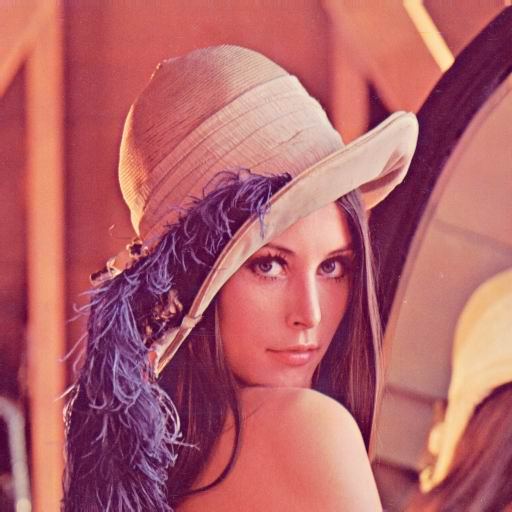
\includegraphics[width=0.9\textwidth]{lenac.png}
        \caption{original}
    \end{subfigure}
    \begin{subfigure}[t]{0.25\textwidth}\centering
        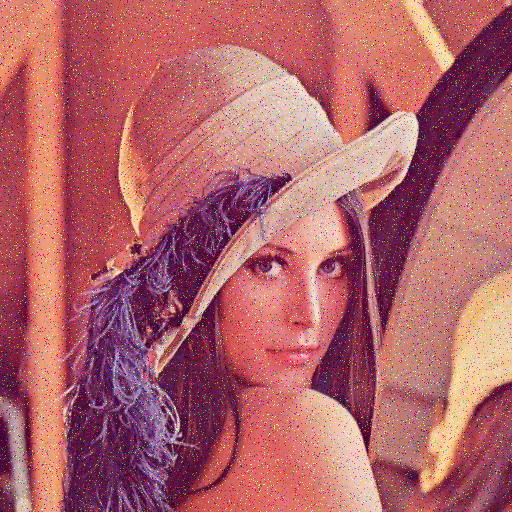
\includegraphics[width=0.9\textwidth]{lenac_impulse3.png}
        \caption{impulse noise}
    \end{subfigure}
    \\[1em]
    \begin{subfigure}[t]{0.2\textwidth}\centering
        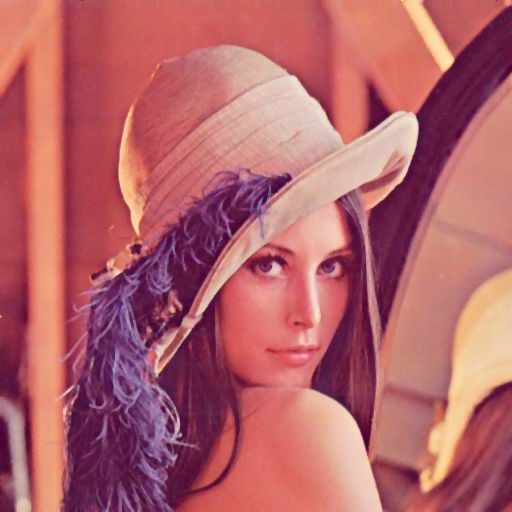
\includegraphics[width=0.9\textwidth]{lenac_impulse_median3.png}
        \caption{median $3\times3$}
    \end{subfigure}
    \begin{subfigure}[t]{0.2\textwidth}\centering
        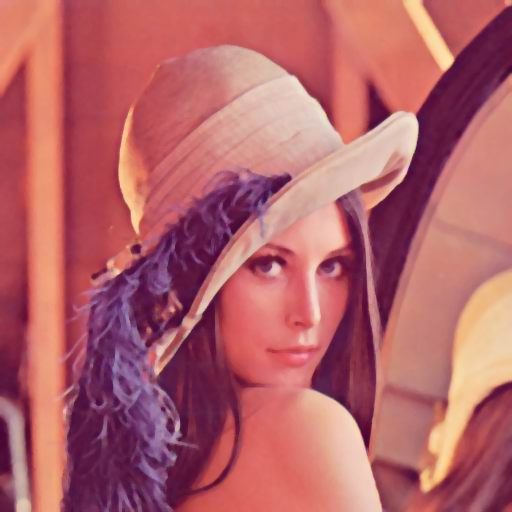
\includegraphics[width=0.9\textwidth]{lenac_impulse_median5.png}
        \caption{median $5\times5$}
    \end{subfigure}
    \begin{subfigure}[t]{0.2\textwidth}\centering
        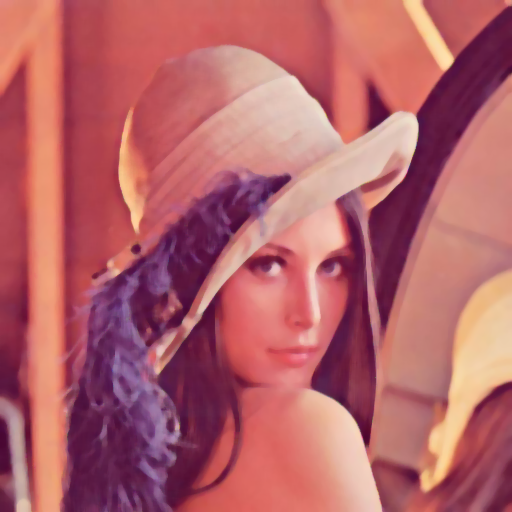
\includegraphics[width=0.9\textwidth]{lenac_impulse_median7.png}
        \caption{median $7\times7$}
    \end{subfigure}
    \begin{subfigure}[t]{0.2\textwidth}\centering
        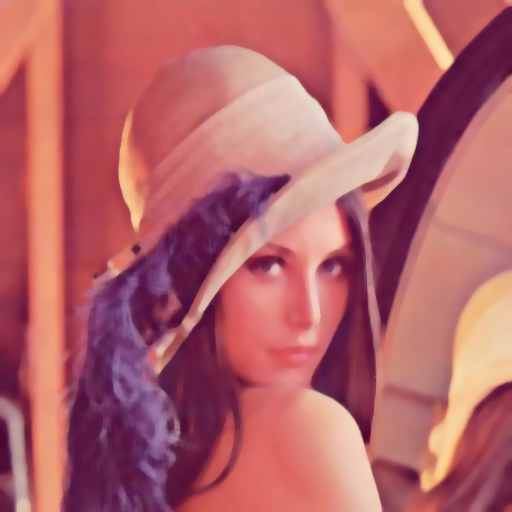
\includegraphics[width=0.9\textwidth]{lenac_impulse_median9.png}
        \caption{median $9\times9$}
    \end{subfigure}
    \caption{Results of denoising the image with the median filter.}
\end{figure}

\begin{table}[H]
    \pgfplotstabletypeset[
        col sep=comma,
        fixed,
        fixed zerofill,
        precision=2,
        every head row/.style ={
                before row = \toprule,
                after row = \midrule
            },
        every last row/.style = {after row =\bottomrule},
        columns/time/.style={column name={\textsc{cpu} time [s]}},
        columns/gpu time/.style={column name={\textsc{gpu} time [s]}, precision=3},
        columns/md/.style={fixed, precision=0},
        columns/operation/.style={string type},
        empty cells with ={---},
    ]{
        operation, time, gpu time, mse, pmse, snr, psnr, md
        none, , , 596.822, 2.340, 11.423, 20.327, 144
        median $3\times3$, 2.286, 0.346, 13.716, 0.054, 27.810, 36.758, 107
        median $5\times5$, 4.814, 0.354, 33.026, 0.130, 23.993, 32.993, 109
        median $7\times7$, 8.289, 0.369, 54.188, 0.213, 21.843, 30.792, 131
        median $9\times9$, 13.417, 0.462, 72.954, 0.286, 20.551, 29.500, 139
    }
    \caption{Time of execution, and coefficients for different parameters of median filter.}
\end{table}

Varying the size of the sampling region, we came to the following conclusions:
Increasing the size of $m$ and $n$ has a noticeable negative impact on the performance of the algorithm on the \textsc{cpu}.
The \textsc{gpu}-accelerated version is so fast, that the performance degradation is negligible.
However, it is not beneficial to increase the size of the sampling region as it is also detrimental to the effectivenes of the denoising.
We can clearly see that the best image was produced by using a $3\times3$ sampling region.
Further increasing its size leads only to producing more blurred image.

Overall, in our opinion, this filter produced a very satisfactory result (at least for this type of noise).
The decrease of the mean square error from 596.82 to 13.72 is a huge improvement,
and our subjective opinion of the produced image is also very positive.

\clearpage
\subsection{Geometric mean filter}

We performed similar parameter analysis for the geometic mean filter.
However, for this experiment we used normal distribution noise in order
to better visualise the differences, because the geometic mean filter
performs very badly with impulse noise (as will be explained in the next section).

\begin{figure}[H]\centering
    \begin{subfigure}[t]{0.25\textwidth}\centering
        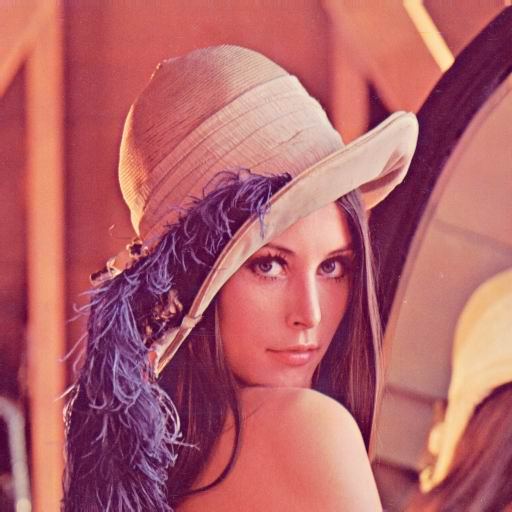
\includegraphics[width=0.9\textwidth]{lenac.png}
        \caption{original}
    \end{subfigure}
    \begin{subfigure}[t]{0.25\textwidth}\centering
        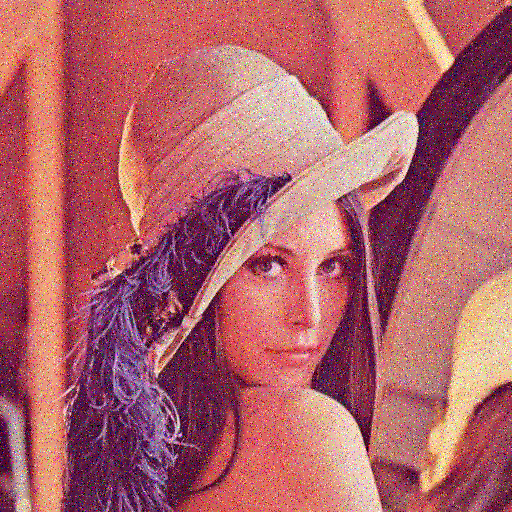
\includegraphics[width=0.9\textwidth]{lenac_normal3.png}
        \caption{normal dist. noise}
    \end{subfigure}
    \\[1em]
    \begin{subfigure}[t]{0.2\textwidth}\centering
        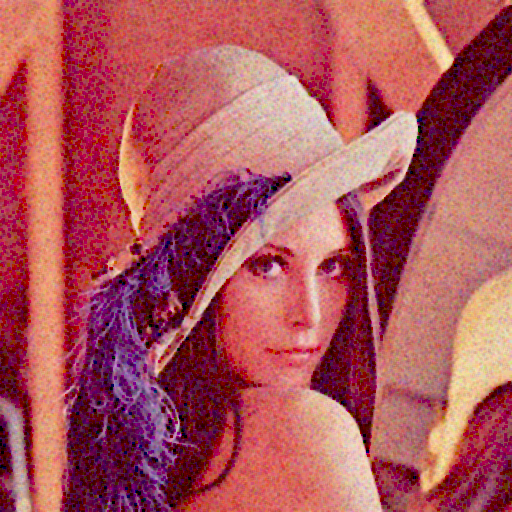
\includegraphics[width=0.9\textwidth]{lenac_normal_gmean3.png}
        \caption{gmean $3\times3$}
    \end{subfigure}
    \begin{subfigure}[t]{0.2\textwidth}\centering
        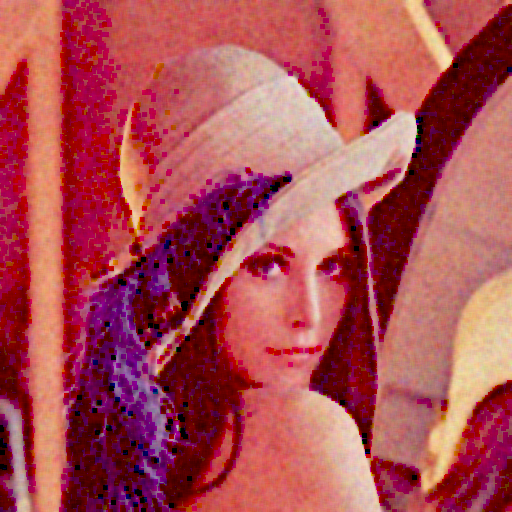
\includegraphics[width=0.9\textwidth]{lenac_normal_gmean5.png}
        \caption{gmean $5\times5$}
    \end{subfigure}
    \begin{subfigure}[t]{0.2\textwidth}\centering
        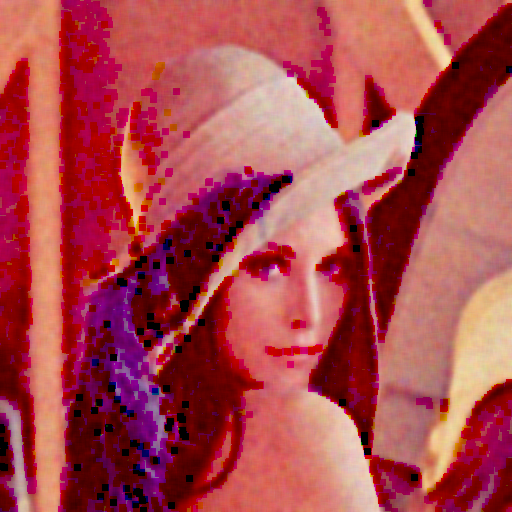
\includegraphics[width=0.9\textwidth]{lenac_normal_gmean7.png}
        \caption{gmean $7\times7$}
    \end{subfigure}
    \begin{subfigure}[t]{0.2\textwidth}\centering
        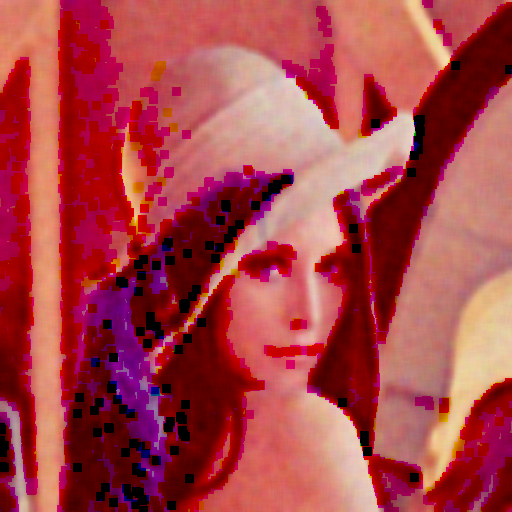
\includegraphics[width=0.9\textwidth]{lenac_normal_gmean9.png}
        \caption{gmean $9\times9$}
    \end{subfigure}
    \caption{Results of denoising the image with the geometric mean filter.}
\end{figure}

\begin{table}[H]\centering
    \pgfplotstabletypeset[
        col sep=comma,
        fixed,
        fixed zerofill,
        precision=2,
        every head row/.style ={
                before row = \toprule,
                after row = \midrule
            },
        every last row/.style = {after row =\bottomrule},
        columns/time/.style={column name={\textsc{cpu} time [s]}},
        columns/gpu time/.style={column name={\textsc{gpu} time [s]}, precision=3},
        columns/md/.style={fixed, precision=0},
        columns/operation/.style={string type},
        empty cells with ={---},
    ]{
        operation, time, gpu time, mse, pmse, snr, psnr, md
        none, , , 755.262, 2.962, 10.401, 19.350, 79
        gmean $3\times3$, 2.140, 0.303, 501.780, 1.986, 12.177, 21.126, 201
        gmean $5\times5$, 3.119, 0.328, 870.211, 3.413, 9.786, 18.753, 221
        gmean $7\times7$, 4.668, 0.330, 1258.318, 4.953, 8.184, 17.133, 234
        gmean $9\times9$, 6.628, 0.313, 1627.559, 6.383, 7.067, 16.015, 241
    }
    \caption{Time of execution, and coefficients for different parameters of gmean filter.}
\end{table}

When it comes to performance, it is immediately noticeable
that increasing the sampling region results in a slower execution when it comes to the \textsc{cpu} implementation.
However, with the \textsc{gpu} implementation a very peculiar thing occurs --- the execution times do not seem to be affected by the change in parameters.
It is contrary to the median filter, where, although very small, a performance degradation was visible.
Out of curiosity, we went for the extreme, and tried this filter with a $100\times100$ sampling region, and were able to achieve execution times as small as 250ms.
Only when we increased the sampling region to $500\times500$ we were able to observe a reproducible performance degradation ($\sim$2s).

Looking at the statistics, we see that increasing the sample region to more than $3\times3$,
the denoised image is actually \emph{worse} than the image with noise
(therefore we're not sure if we can even call the produced image ``denoised'').
Even if there is some improvement produced by the $3\times3$ gmean filter, it is very slight.
Looking at the produced image, there is still visible noise, and the image is noticeably darker.

However, one interesting things that we noticed is that the filter seems to ``highlight'' a certain features of the picture.
For example, expecially visible at the $7\times7$ result image, there are some very intense red artifacts produced around the model's lips and eyes.

Overall, our impression is that this filter, although fast, yields significantly worse results than the median filter.
Especially with larger sampling regions, it produces weird artifacts and is very destructive to the image.

\section{Analysis of the parameters of the noise reduction methods}

To better understand which filter is best suited to which type of noise,
oth of the median and gmean filters was tested on 3 types of noise --- uniform, normal, and impulse.

\subsubsection{Median filter}

\begin{figure}[h]\centering
    \begin{subfigure}[t]{.4\textwidth}\centering
        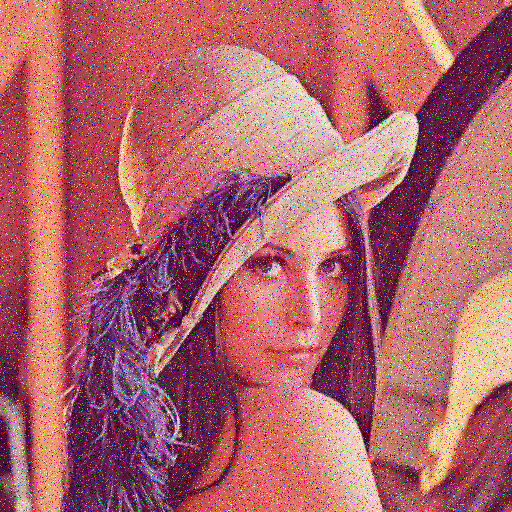
\includegraphics[width=.8\textwidth]{lenac_uniform3}
        \caption{Image with uniform noise}
    \end{subfigure}
    \begin{subfigure}[t]{.4\textwidth}\centering
        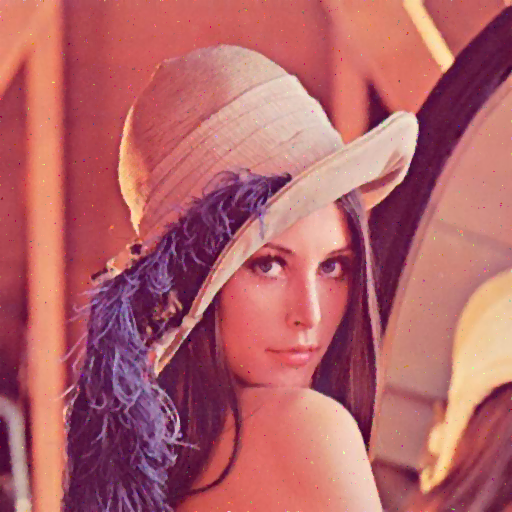
\includegraphics[width=.8\textwidth]{lenac_uniform_median}
        \caption{Uniform noise after median $3\times3$}
    \end{subfigure}\\[2em]
    \begin{subfigure}[t]{.4\textwidth}\centering
        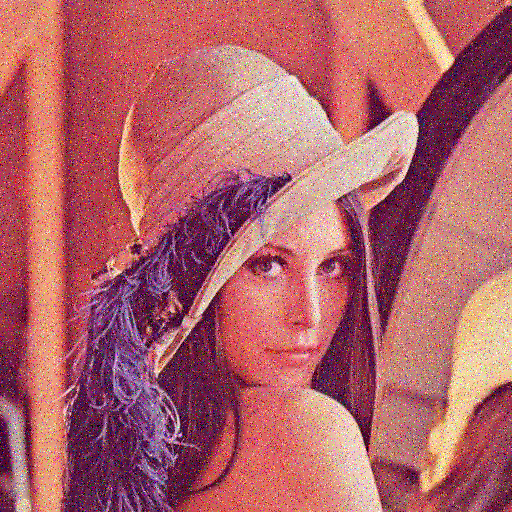
\includegraphics[width=.8\textwidth]{lenac_normal3}
        \caption{Image with normal noise}
    \end{subfigure}
    \begin{subfigure}[t]{.4\textwidth}\centering
        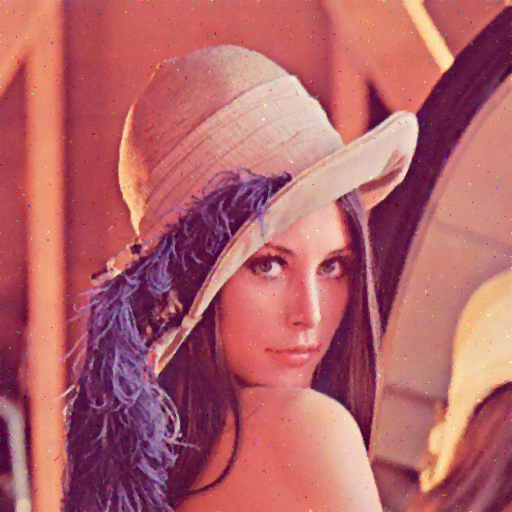
\includegraphics[width=.8\textwidth]{lenac_normal_median}
        \caption{Normal noise after median $3\times3$}
    \end{subfigure}\\[2em]
    \begin{subfigure}[t]{.4\textwidth}\centering
        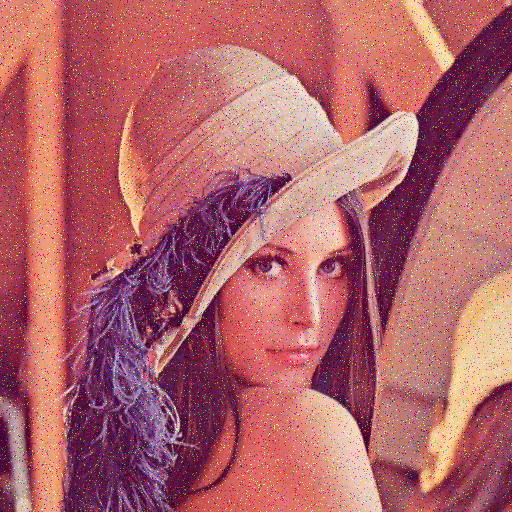
\includegraphics[width=.8\textwidth]{lenac_impulse3}
        \caption{Image with impulse noise}
    \end{subfigure}
    \begin{subfigure}[t]{.4\textwidth}\centering
        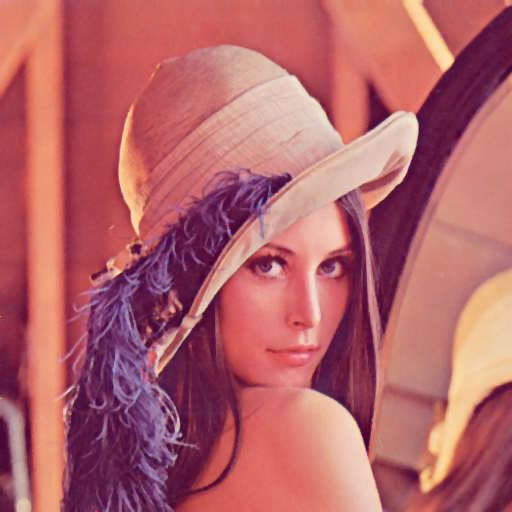
\includegraphics[width=.8\textwidth]{lenac_impulse_median}
        \caption{Impulse noise after median $3\times3$}
    \end{subfigure}
    \caption{Results of running $3\times3$ median filter on different types of noise}
\end{figure}

\begin{table}[h]\centering
    \pgfplotstabletypeset[
        col sep=&,
        row sep=\\,
        fixed,
        fixed zerofill,
        precision=2,
        every head row/.style ={
                before row = \toprule,
                after row = \midrule[1pt]
            },
        every last row/.style = {after row =\bottomrule},
        columns/operation/.style={string type, column type={l}},
        columns/noise type/.style={string type,
                assign cell content/.code={%
                        \pgfmathparse{int(Mod(\pgfplotstablerow,2))}%
                        \ifnum\pgfmathresult=0%
                            \pgfkeyssetvalue{/pgfplots/table/@cell content}%
                            {\multirow{2}{*}{##1}}%
                        \else
                            \pgfkeyssetvalue{/pgfplots/table/@cell content}%
                            {\phantom{.}}%
                        \fi%
                    },},
        columns/md/.style={fixed, precision=0},
        every odd row/.style = {after row=\midrule[0.1pt]},
        empty cells with ={---},
    ]
    {
        operation         & noise type & mse & pmse & snr & psnr & md \\
        none              & uniform    & 1203.271     & 4.719         & 8.378        & 17.327        & 152         \\
        median $3\times3$ & uniform    & 33.660       & 0.132         & 23.911       & 32.860        & 123         \\
        none              & normal     & 755.262      & 2.962         & 10.401       & 19.350        & 79          \\
        median $3\times3$ & normal     & 42.337       & 0.166         & 22.915       & 31.864        & 92          \\
        none              & impulse    & 596.822      & 2.340         & 11.423       & 20.372        & 144         \\
        median $3\times3$ & impulse    & 13.716       & 0.054         & 27.810       & 36.758        & 107         \\
    }
    \caption{Results of running $3\times3$ median filter on different types of noise}
    \label{tab:median-noise-results}
\end{table}

From table \ref{tab:median-noise-results}, we clearly see that the median filter performs best with the impulse noise.
This was to be expected, as the characteristic of the impulse noise is that it is either minimum or maximum intensity.
Therefore, the probability of it being a median is very low.
On the contrary, normal distribution noise,
has a much higher probability of being a median,
therefore, the median filter performs much more poorly.

When it comes to subjective visual impressions,
In our opinion, the median filter performed very well.
In case of the impulse noise, the produced image is very clear, without any visible noise.
In case of the uniform and normal noises, there are some tiny specs of noise still visible,
however, the image after filtering is still much clearer than the unfiltered nois

\clearpage
\subsubsection{Geometric mean filter}

\begin{figure}[h]\centering
    \begin{subfigure}[t]{.4\textwidth}\centering
        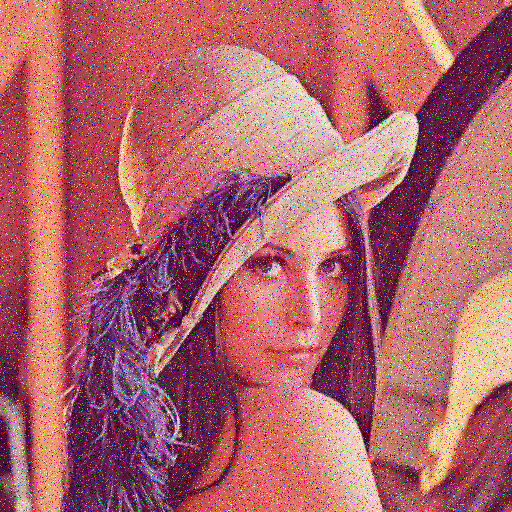
\includegraphics[width=.8\textwidth]{lenac_uniform3}
        \caption{Image with uniform noise}
    \end{subfigure}
    \begin{subfigure}[t]{.4\textwidth}\centering
        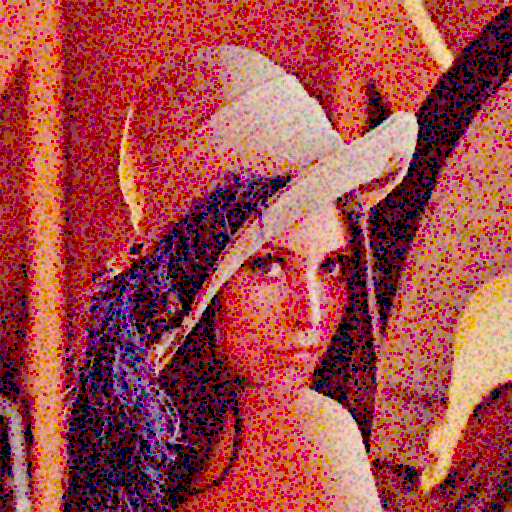
\includegraphics[width=.8\textwidth]{lenac_uniform_gmean}
        \caption{Uniform noise after gmean $3\times3$}
    \end{subfigure}\\[2em]
    \begin{subfigure}[t]{.4\textwidth}\centering
        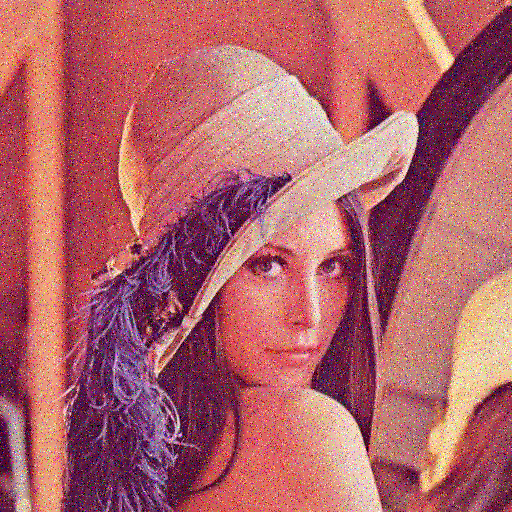
\includegraphics[width=.8\textwidth]{lenac_normal3}
        \caption{Image with normal noise}
    \end{subfigure}
    \begin{subfigure}[t]{.4\textwidth}\centering
        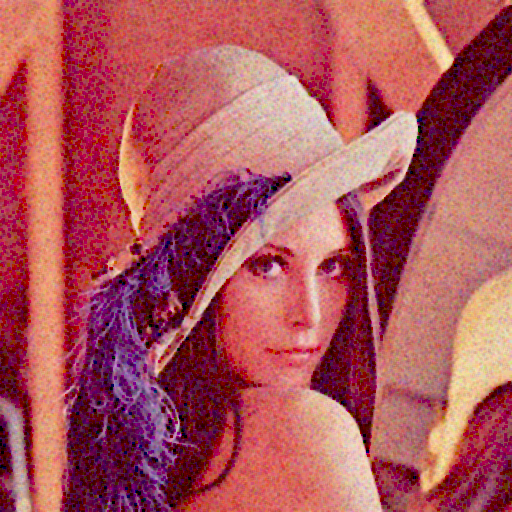
\includegraphics[width=.8\textwidth]{lenac_normal_gmean}
        \caption{Normal noise after gmean $3\times3$}
    \end{subfigure}\\[2em]
    \begin{subfigure}[t]{.4\textwidth}\centering
        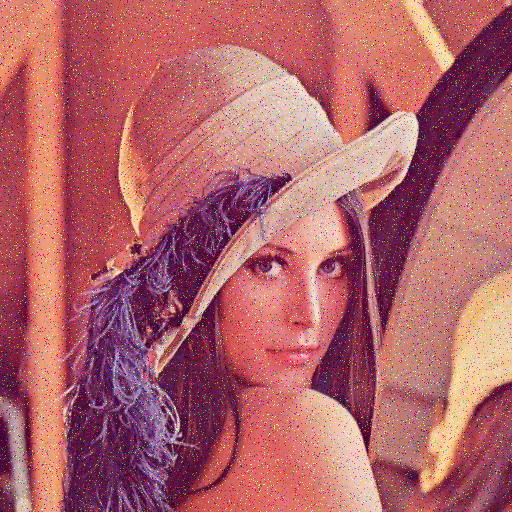
\includegraphics[width=.8\textwidth]{lenac_impulse3}
        \caption{Image with impulse noise}
    \end{subfigure}
    \begin{subfigure}[t]{.4\textwidth}\centering
        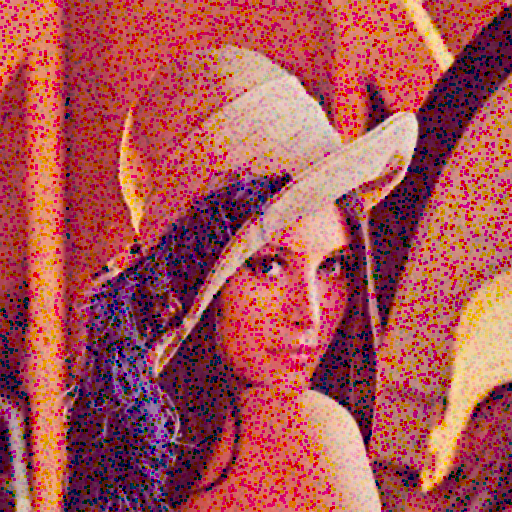
\includegraphics[width=.8\textwidth]{lenac_impulse_gmean}
        \caption{Impulse noise after gmean $3\times3$}
    \end{subfigure}
    \caption{Results of running $3\times3$ geometic mean filter on different types of noise}
\end{figure}

\begin{table}[h]\centering
    \pgfplotstabletypeset[
        col sep=&,
        row sep=\\,
        fixed,
        fixed zerofill,
        precision=2,
        every head row/.style ={
                before row = \toprule,
                after row = \midrule[1pt]
            },
        every last row/.style = {after row =\bottomrule},
        columns/operation/.style={string type, column type={l}},
        columns/noise type/.style={string type,
                assign cell content/.code={%
                        \pgfmathparse{int(Mod(\pgfplotstablerow,2))}%
                        \ifnum\pgfmathresult=0%
                            \pgfkeyssetvalue{/pgfplots/table/@cell content}%
                            {\multirow{2}{*}{##1}}%
                        \else
                            \pgfkeyssetvalue{/pgfplots/table/@cell content}%
                            {\phantom{.}}%
                        \fi%
                    },},
        columns/md/.style={fixed, precision=0},
        every odd row/.style = {after row=\midrule[0.1pt]},
        empty cells with ={---},
    ]
    {
        operation         & noise type & mse & pmse & snr & psnr & md \\
        none              & uniform    & 1203.271     & 4.719         & 8.378        & 17.327        & 152         \\
        gmean $3\times3$  & uniform    & 1807.199     & 7.087         & 6.612        & 15.561        & 213         \\
        none              & normal     & 755.262      & 2.962         & 10.401       & 19.350        & 79          \\
        gmean $3\times3$  & normal     & 501.780      & 1.968         & 12.177       & 21.126        & 201         \\
        none              & impulse    & 596.822      & 2.340         & 11.423       & 20.372        & 144         \\
        gmean $3\times3$  & impulse    & 1347.598     & 5.285         & 7.886        & 16.835        & 220         \\
    }
    \caption{Results of running $3\times3$ geometic mean filter on different types of noise}
    \label{tab:gmean-noise-results}
\end{table}

From table \ref{tab:gmean-noise-results} is is immediately noticeable
that the geometric mean filter performs nowhere near as well as the median filter.

The only type of noise that it did improve in terms of objective coefficients, is the normal dist.\ noise.
In uniform and impulse noise, the image after filtering was actually \emph{worse} than the original image.

We believe that is the case because the geometric mean filter has a very big weakness when it encounters a pixel with a luminosity of 0.
That is, because 0 is the absorbing element of multiplication, i.e.\ any number multiplied by 0 is 0.
That means, that if there is a pixel with luminosity 0, the geometric mean in all pixels in the neighbourhood of that pixel will have their geometric mean computed to 0.

The probability of a noise pixel having 0 luminosity is the highest for the impulse noise,
and the lowest for the normal dist. noise.
This is why, the geometric mean filter with this types has the worst and best performance respectively.

The result of this peculiar behavoiur with 0 luminosity pixels, causes the geometric mean to produce weird looking artifacts.
These manifest as colorful rectangles (usually red,green,blue,yellow,magenta or cyan) on the color image.
With the monochrome image,
these would show as completely black rectangles.
The dimensions of these rectangles is determined by the size of the filter's samplling region.

Our visual impressions is that the geometric filter yields unsatisfactory results.
In case of gaussian noise, there are some improvements, but still worse than with the median filter.
In case of uniform and impulse noise, the results are an absolute tragedy. The produced pictures are full of the abovementioned artifacts,
which results in the output image being more noisy than the input.
Additionally, the produced images are noticeably darker.

Overall, we conclude that the median filter performs best with the impulse noise, and the geometric mean filter is best suited for dealing wth gaussian noise.

\clearpage
\vfill
\section*{Teacher's remarks}
\begin{tabularx}{\textwidth}{|X|}
    \hline
    \vspace{7cm}
    \phantom{.} \\
    \hline
\end{tabularx}

\end{document}